\documentclass[10pt,journal]{IEEEtran}
\usepackage{graphicx,booktabs,amsmath,url,cite,multirow}
\usepackage[hidelinks]{hyperref}

\begin{document}

\title{An End-to-End Computer-Vision and LLM Pipeline for Badminton Singles Analytics: Court-Calibrated Tracking, SlowFast Shot Recognition and Natural-Language Coaching}

\author{Divya Prakash%
\thanks{Corresponding author. Code: \url{https://github.com/divyaprakash0426/badminton-ai}.}}

\maketitle

\begin{abstract}
Badminton analytics is usually either manual (annotated stroke-level datasets) or limited to a single perception task. We describe an open, end-to-end system that turns a single-camera singles video into court-calibrated statistics and natural-language coaching feedback. A four-point homography maps image coordinates to BWF court metres; YOLO11-pose tracks players, TrackNetV3 with inpainting tracks the shuttlecock, hits are segmented into rallies, each stroke is classified by a SlowFast R50 network fine-tuned on VideoBadminton (18 classes), and a compact match summary is passed to a large language model that returns structured JSON feedback and answers follow-up questions in an interactive dashboard. On the VideoBadminton validation split (1{,}558 clips) the classifier reaches 86.5\% top-1 accuracy (95\% CI 84.7--88.2) and 0.80 macro-F1, at 40\,ms per clip on a laptop GPU, and the detection pipeline runs at about 30 frames/s on the same GPU. We state plainly what is \emph{not} validated: the split is clip-level, so players and scenes overlap between training and evaluation; rally segmentation, scoring and distance statistics have no ground truth; and LLM feedback is checked only for consistency with detected shot labels (26 of 27 cited shot terms consistent). The contribution is a reproducible integration and an honest baseline for end-to-end evaluation rather than a new model.
\end{abstract}

\begin{IEEEkeywords}
badminton, sports analytics, action recognition, SlowFast, shuttlecock tracking, homography, large language models
\end{IEEEkeywords}

\section{Introduction}
Tactical analysis in badminton relies on stroke-level records of shot type, landing zone and rally outcome. Public datasets such as ShuttleSet \cite{wang2023shuttleset} provide such annotations, but producing them for new matches is labour intensive. Component technologies now exist for each perception step: shuttlecock tracking \cite{huang2019tracknet,chen2023tracknetv3}, pose estimation \cite{jocher2024ultralytics} and stroke recognition on VideoBadminton \cite{li2024videobadminton}. What a coach or player needs, however, is a single tool that connects them, expresses results in court coordinates, and explains them in plain language.

We present such a tool and evaluate it as far as available data allow. Our contributions are:
\begin{enumerate}
\item an end-to-end architecture combining homography-based court calibration, concurrent YOLO11-pose and TrackNetV3 processing, SlowFast shot classification, per-player movement analytics and a rule-based score estimate;
\item an LLM coaching module that consumes a compact structured summary and returns schema-constrained JSON (match summary, opponent weaknesses, improvements, drills, per-rally critiques) plus grounded question answering;
\item a re-evaluation of the fine-tuned SlowFast classifier with bootstrap confidence intervals, latency and per-class analysis, together with a candid account of the evaluation-protocol limits;
\item an open-source Streamlit dashboard and regression tests.
\end{enumerate}
We do not claim state-of-the-art recognition accuracy; Section~\ref{sec:limits} lists what remains to be validated.

\section{Related Work}
\textbf{Badminton datasets.} ShuttleSet \cite{wang2023shuttleset} offers human-annotated stroke-level singles data for tactical modelling; the earlier Badminton Coach AI platform \cite{wang2020badminton} demonstrated deep-learning-based match analysis. VideoBadminton \cite{li2024videobadminton} provides trimmed clips labelled with 18 stroke classes and reports SlowFast and other baselines.\\
\textbf{Shuttlecock tracking.} TrackNet \cite{huang2019tracknet} introduced heat-map regression over stacked frames for small, fast objects; TrackNetV3 \cite{chen2023tracknetv3} adds background estimation, mixup and a trajectory-rectification (inpainting) module. We use the released implementation.\\
\textbf{Video recognition.} SlowFast \cite{feichtenhofer2019slowfast} processes a slow, spatially rich pathway and a fast, lightweight temporal pathway. We use the PyTorchVideo \cite{fan2021pytorchvideo} R50 model pretrained on Kinetics-400 \cite{kay2017kinetics}.\\
\textbf{LLMs in sports feedback.} Multimodal LLMs \cite{gemini2023} can generate fluent feedback, but need factual conditioning; we feed the model only structured statistics produced by the vision pipeline.

\section{System Architecture}
Fig.~\ref{fig:arch} shows the pipeline. A single pass decodes the video once and feeds YOLO11x-pose and TrackNetV3 concurrently, avoiding repeated decoding. The user marks the four corners of the singles court in a calibration frame of the dashboard; the resulting homography $H$ \cite{hartley2004multiple} maps pixel coordinates to metres in the BWF court frame, so player positions, shuttle landings and speeds are metric and zone-labelled. Hits are segmented from the tracked shuttle trajectory and player positions, and consecutive hits are grouped into rallies. For each hit a 2\,s clip is cropped and classified by the SlowFast network. A rule-based scorer estimates the rally winner from landing position (in/out) and last hitter. Aggregates are summarised and sent to the LLM coach.

\begin{figure*}[t]
\centering
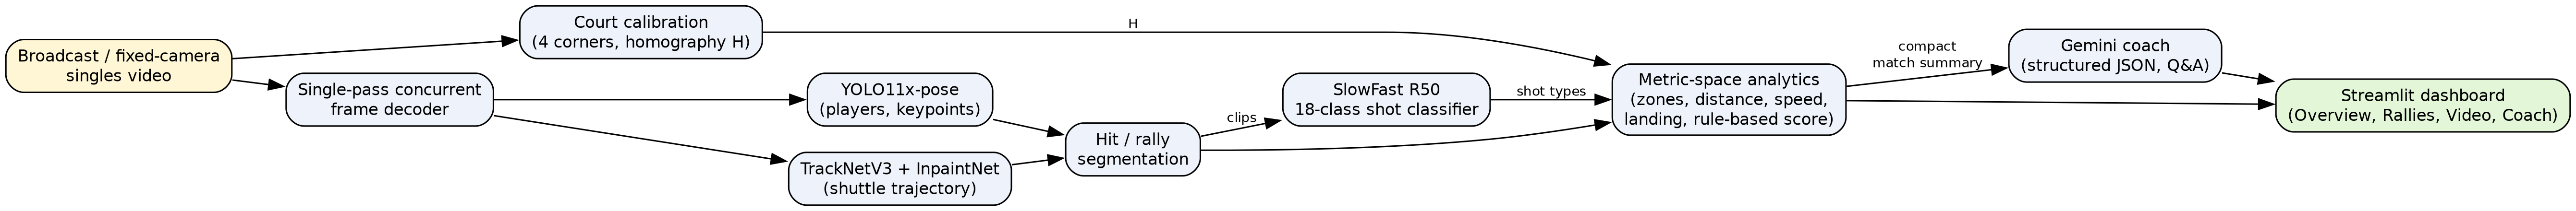
\includegraphics[width=\textwidth]{figures/architecture.png}
\caption{System architecture. Calibration provides the homography $H$; vision modules run concurrently over a single decode pass and feed a metric-space analytics layer whose summary conditions the LLM coach and the dashboard.}
\label{fig:arch}
\end{figure*}

\section{Methods}
\subsection{Shot classifier}
The classifier is SlowFast R50 initialised from Kinetics-400 with the final projection replaced by an 18-way linear layer. Inputs are 32 uniformly sampled frames from a 2.0\,s clip, short side scaled to 256 (random crop 256 and horizontal flip in training), normalised with mean 0.45 and std 0.225; the slow pathway uses every fourth frame ($\alpha=4$). Training used SGD (momentum 0.9, weight decay $10^{-4}$), learning rate 0.01 with cosine decay, mixed precision and batch size 32 on the 6{,}264-clip training split; the released checkpoint is evaluated. No training was performed for this paper; we re-evaluate the released checkpoint.

\subsection{LLM coach}
The coach receives a compact JSON summary (score progression, shot distribution, per-player distance and speed, per-rally shot sequences and winner) and is asked, in JSON mode, for a fixed schema with keys \emph{match\_summary}, \emph{opponent\_weakness}, \emph{my\_improvements}, \emph{drills} and \emph{rally\_critiques}. The model name is configurable (here Gemini 3.8 Flash); on failure the module degrades to a safe message, and API keys are redacted from errors. A chat interface answers follow-up questions conditioned on the same summary.

\section{Experiments}
\subsection{Shot recognition}
\textbf{Protocol.} We evaluate on the local validation split of VideoBadminton (1{,}558 clips, 18 classes) using the same transform as in training, uniform 2\,s clip sampling, and an RTX 4080 Laptop GPU (fp32). Confidence intervals are percentile bootstrap (2{,}000 resamples) over clips. The script is \texttt{paper/experiments/eval\_slowfast.py}.

\textbf{Results.} Top-1 accuracy is 86.5\% (95\% CI 84.7--88.2), top-5 98.3\%, macro-F1 0.799 (0.769--0.825), weighted-F1 0.863 and mean per-class accuracy 78.9\%. Inference takes 39.9\,ms per clip at batch size 1. Table~\ref{tab:cls} lists per-class scores; serves, clears, drops and smashes exceed 0.88 F1, while Tap Smash (0.44), Push Shot (0.61), Transitional Slice (0.53) and Defensive Clear (0.68) are weakest. These are mostly rare classes (21--24 validation clips) or classes visually close to a neighbour (Fig.~\ref{fig:cm}); Tap Smash has perfect precision but 0.29 recall.

\begin{table}[t]
\centering\caption{Per-class results on the validation split.}\label{tab:cls}
\small
\begin{tabular}{lcccr}
\toprule
Class & P & R & F1 & $n$\\
\midrule
Short Serve & 0.97 & 0.99 & 0.98 & 176\\
Long Serve & 0.98 & 0.99 & 0.98 & 198\\
Clear & 0.96 & 0.91 & 0.93 & 189\\
Short Flat Shot & 1.00 & 0.85 & 0.92 & 26\\
Defensive Drive & 0.95 & 0.86 & 0.90 & 22\\
Drop Shot & 0.91 & 0.88 & 0.89 & 162\\
Smash & 0.84 & 0.94 & 0.89 & 164\\
Rear Court Flat Drive & 0.95 & 0.83 & 0.89 & 24\\
Lift & 0.83 & 0.85 & 0.84 & 151\\
Cut & 0.86 & 0.81 & 0.83 & 117\\
Rush Shot & 0.77 & 0.91 & 0.83 & 22\\
Cross Court Flight & 0.74 & 0.76 & 0.75 & 33\\
Block & 0.68 & 0.83 & 0.75 & 63\\
Flat Shot & 0.71 & 0.78 & 0.74 & 65\\
Defensive Clear & 0.76 & 0.62 & 0.68 & 21\\
Push Shot & 0.64 & 0.57 & 0.61 & 80\\
Transitional Slice & 0.52 & 0.54 & 0.53 & 24\\
Tap Smash & 1.00 & 0.29 & 0.44 & 21\\
\bottomrule
\end{tabular}
\end{table}

\begin{figure}[t]
\centering
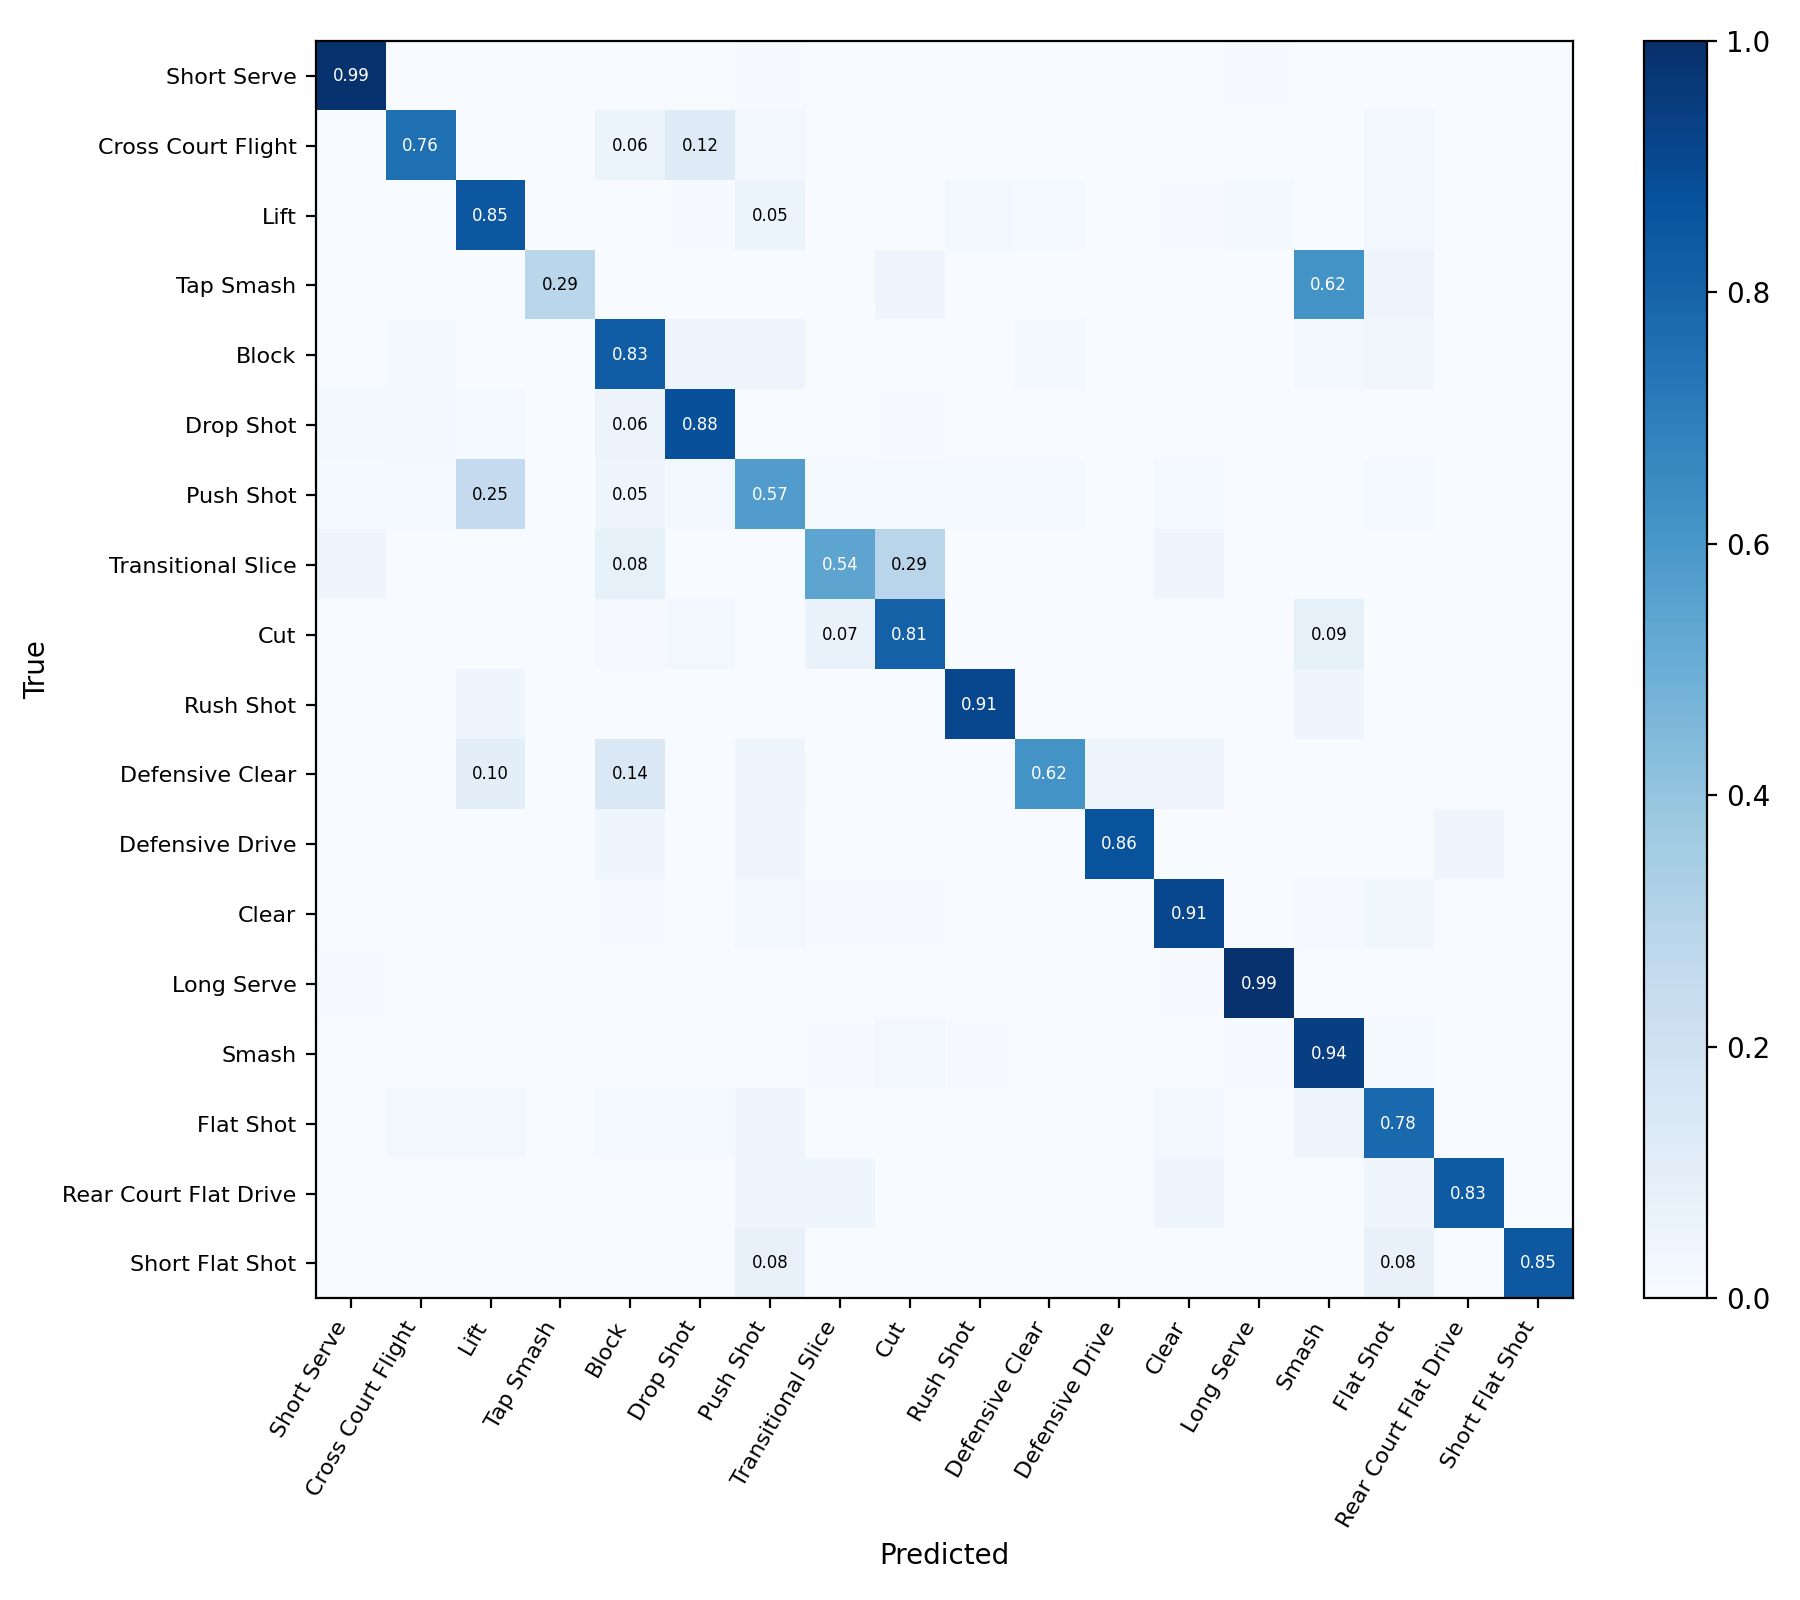
\includegraphics[width=\columnwidth]{figures/confusion_matrix.png}
\caption{Row-normalised confusion matrix (cells $\ge 0.05$ annotated).}
\label{fig:cm}
\end{figure}

\subsection{Full-pipeline run}
We processed a 184\,s Paris 2024 broadcast highlight (1280$\times$720, 25\,fps) with a user-specified court quadrilateral. The pipeline detected 14 rallies and 120 shots (mean 8.6 shots per rally; 24 shots labelled ``Unknown''). Dominant predicted classes were Defensive Clear (42) and Serve (14). Estimated per-player distances were 440\,m (Near) and 451\,m (Far). Separately, processing a 40\,s clip (1{,}000 frames) took about 33\,s on the same GPU, i.e.\ about 30 frames/s. The reel is an edited highlight containing cuts and a scoreboard spanning several games, so its on-screen score cannot be used as ground truth for our per-rally score estimate; we therefore make no accuracy claim for rally segmentation or scoring.

\subsection{LLM feedback consistency}
On the 14 detected rallies we asked the coach for per-rally critiques and counted shot-type terms (e.g., smash, drop, clear) cited in each critique that actually appear among the detected shots of that rally. 26 of 27 cited terms (96\%) were consistent. This measures agreement with the \emph{pipeline's labels}, not correctness against the real match, and does not assess the usefulness of the advice; some critiques also assert qualitative outcomes (e.g., ``unforced error'') that the structured summary cannot support. A user study with coaches is required before any claim of pedagogical value.

\section{Interface}
The Streamlit dashboard (Figs.~\ref{fig:ui1} and \ref{fig:ui2}) walks the user through upload, calibration, processing and results (Overview, Rallies, Video and AI Coach tabs) with a dark ``kinetic telemetry'' theme designed with Stitch.

\begin{figure}[t]
\centering
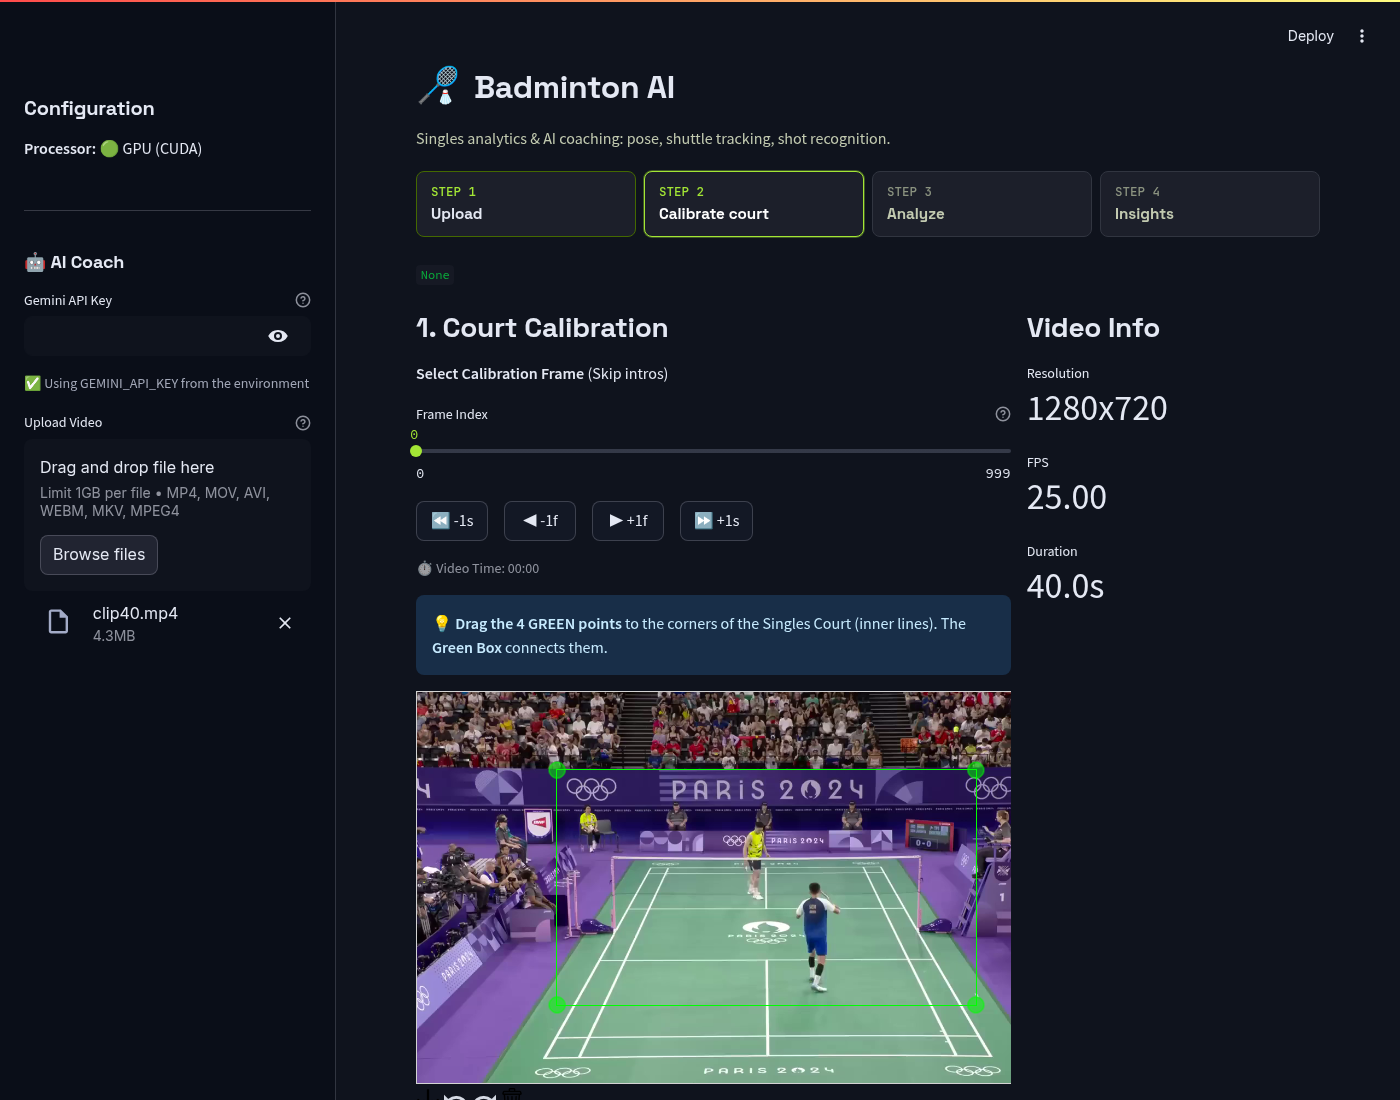
\includegraphics[width=\columnwidth]{figures/ui_calibration.png}
\caption{Calibration step: the user drags four corner markers onto the singles court.}
\label{fig:ui1}
\end{figure}
\begin{figure}[t]
\centering
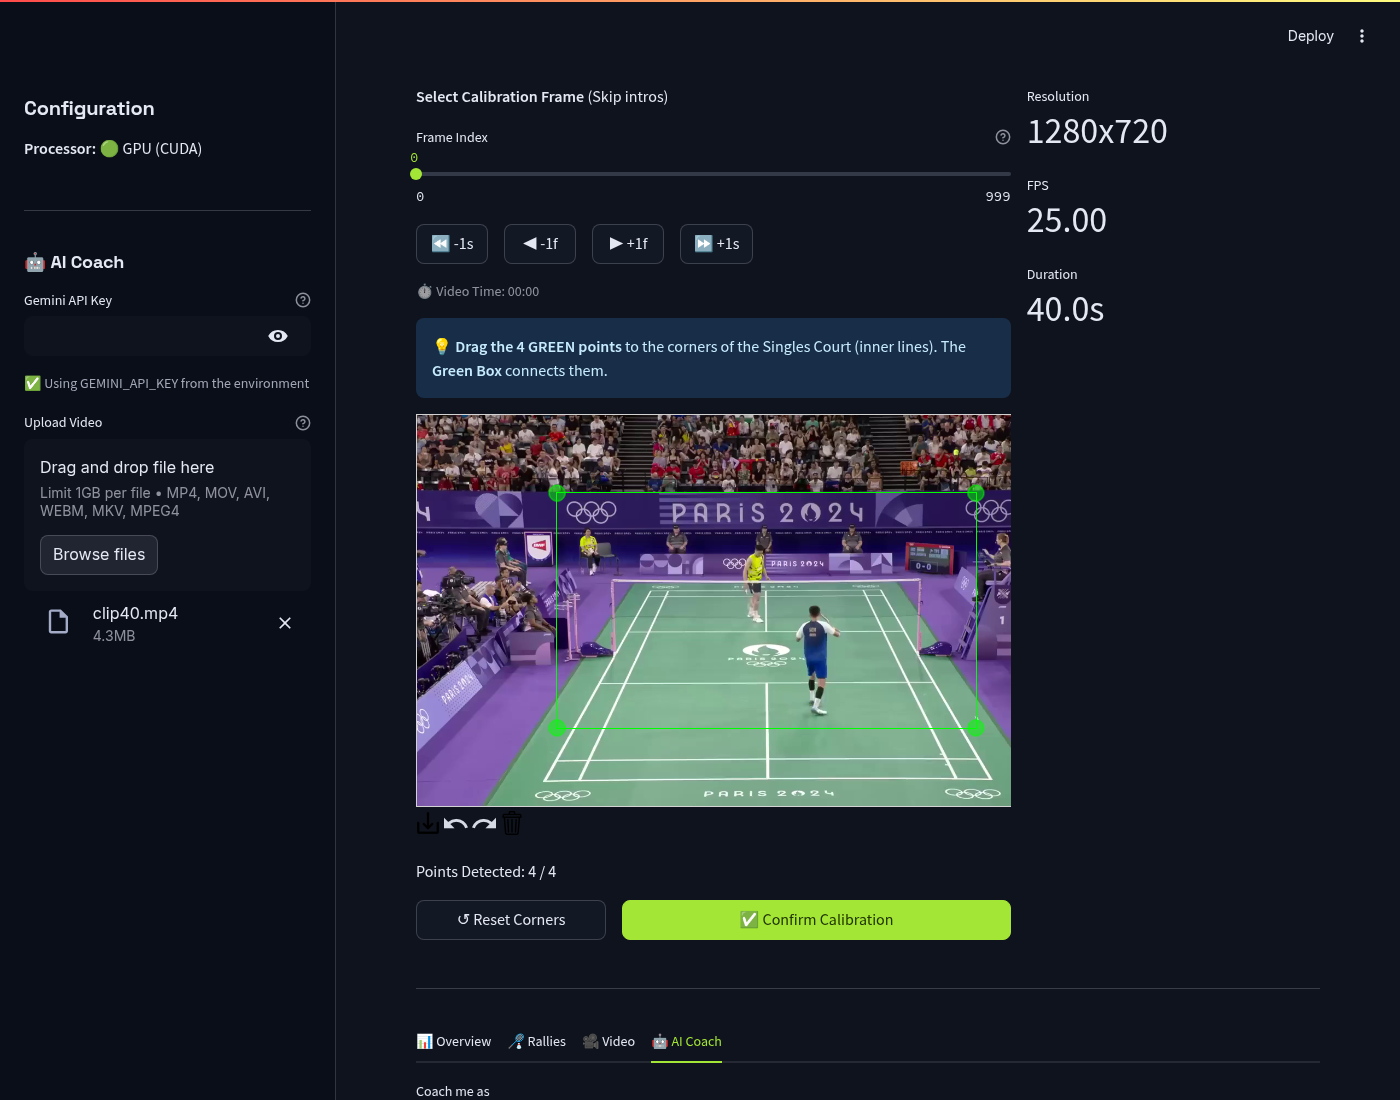
\includegraphics[width=\columnwidth]{figures/ui_coach.png}
\caption{Results dashboard with the AI Coach tab.}
\label{fig:ui2}
\end{figure}

\section{Limitations and Threats to Validity}\label{sec:limits}
\begin{itemize}
\item \textbf{Split leakage.} The dataset was split 80/20 at clip level; all 77 validation recording sessions also occur in training. Players, courts and cameras are therefore shared, and the reported accuracy is optimistic for unseen matches. There is no separate test set, and checkpoint selection used the same validation split. Our numbers are not comparable to those reported by the dataset authors \cite{li2024videobadminton}.
\item \textbf{Domain shift.} VideoBadminton is recorded in a specific setting; on the broadcast clip, 20\% of shots were labelled ``Unknown'' (and many others had low classifier confidence), and the predicted class distribution (many Defensive Clear) suggests systematic bias. We did not label broadcast strokes, so cross-domain accuracy is unknown.
\item \textbf{Unvalidated analytics.} Rally segmentation, winner and score estimates, distances and speeds lack ground truth. Peak speeds (up to 15\,m/s) exceed plausible human sprint speeds, indicating tracking or homography noise; distances should be treated as indicative.
\item \textbf{Calibration dependence.} Metric outputs depend on manual corner placement and a stable camera.
\item \textbf{LLM.} Output is model-dependent and non-deterministic; feasibility of consistency is shown, correctness is not.
\end{itemize}

\section{Conclusion and Future Work}
We assembled and open-sourced an end-to-end badminton analysis pipeline that couples established vision models with metric calibration and an LLM coach, and reported a transparent re-evaluation of its stroke classifier. The next steps required for a rigorous claim are a session-disjoint evaluation of the classifier, a hand-annotated end-to-end benchmark (rally boundaries, winners, landings), evaluation of speed and distance against known references, ablations (e.g., without TrackNet inpainting or dynamic zone assignment), and a coach/player study of the generated feedback.

\section*{Acknowledgment}
The shot classifier was trained on VideoBadminton; TrackNetV3 weights and code are from their authors. The Gemini model was used under the author's API access.

\bibliographystyle{IEEEtran}
\bibliography{references}
\end{document}
